% This is the Duke University Statistical Science LaTeX thesis template.
% It has been adapted from the Reed College LaTeX thesis template. The
% adaptation was done by Mine Cetinkaya-Rundel (MCR). Some of the comments
% that are specific to Reed College have been removed.
%
% Most of the work on the original Reed College document class and template
% was done by Sam Noble (SN). Later comments etc. by Ben Salzberg (BTS).
% Additional restructuring and APA support by Jess Youngberg (JY).
%
% See https://www.reed.edu/cis/help/latex/ for help. There are a
% great bunch of help pages there, with notes on
% getting started, bibtex, etc. Go there and read it if you're not
% already familiar with LaTeX.
%
% Any line that starts with a percent symbol is a comment.
% They won't show up in the document, and are useful for notes
% to yourself and explaining commands.
% Commenting also removes a line from the document;
% very handy for troubleshooting problems. -BTS

%%
%% Preamble
%%
% \documentclass{<something>} must begin each LaTeX document
\documentclass[12pt,twoside]{dukestatscithesis}
% Packages are extensions to the basic LaTeX functions. Whatever you
% want to typeset, there is probably a package out there for it.
% Chemistry (chemtex), screenplays, you name it.
% Check out CTAN to see: http://www.ctan.org/
%%
\usepackage{graphicx,latexsym}
\usepackage{amsmath}
\usepackage{amssymb,amsthm}
\usepackage{longtable,booktabs,setspace}
\usepackage{chemarr} %% Useful for one reaction arrow, useless if you're not a chem major
\usepackage[hyphens]{url}
% Added by CII
\usepackage{hyperref}
\usepackage{lmodern}
\usepackage{float}
\floatplacement{figure}{H}
% End of CII addition
\usepackage{rotating}

% Next line commented out by CII
%%% \usepackage{natbib}
% Comment out the natbib line above and uncomment the following two lines to use the new
% biblatex-chicago style, for Chicago A. Also make some changes at the end where the
% bibliography is included.
%\usepackage{biblatex-chicago}
%\bibliography{thesis}


% Added by CII (Thanks, Hadley!)
% Use ref for internal links
\renewcommand{\hyperref}[2][???]{\autoref{#1}}
\def\chapterautorefname{Chapter}
\def\sectionautorefname{Section}
\def\subsectionautorefname{Subsection}
% End of CII addition

% Added by CII
\usepackage{caption}
\captionsetup{width=5in}
% End of CII addition

% \usepackage{times} % other fonts are available like times, bookman, charter, palatino


% To pass between YAML and LaTeX the dollar signs are added by CII
\title{Tensor Completion Techniques For Anomaly Detection in Network Attacks}
\author{James C. Wu}
% The month and year that you submit your FINAL draft TO THE LIBRARY (May or December)
\date{May 2018}
\advisor{Peter D. Hoff}
\institution{Duke University}
\degree{Bachelor of Science in Statistical Science}
\committeememberone{Committeemember O. Name}
\committeemembertwo{Committeemember T. Name}
\dus{Mine Cetinkaya-Rundel}
%If you have two advisors for some reason, you can use the following
% Uncommented out by CII
% End of CII addition

%%% Remember to use the correct department!
\department{Department of Statistical Science}

% Added by CII
%%% Copied from knitr
%% maxwidth is the original width if it's less than linewidth
%% otherwise use linewidth (to make sure the graphics do not exceed the margin)
\makeatletter
\def\maxwidth{ %
  \ifdim\Gin@nat@width>\linewidth
    \linewidth
  \else
    \Gin@nat@width
  \fi
}
\makeatother

\renewcommand{\contentsname}{Table of Contents}
% End of CII addition

\setlength{\parskip}{0pt}

% Added by CII
  %\setlength{\parskip}{\baselineskip}
  \usepackage[parfill]{parskip}

\providecommand{\tightlist}{%
  \setlength{\itemsep}{0pt}\setlength{\parskip}{0pt}}

\Acknowledgements{
I thank my advisor, Professor Peter Hoff, and the Director of
Undergraduate Studies, Professor Mine Cetinkaya-Rundel, for their
guidance in this project. I also thank Duke University's Statistics
Department and Office of Information Technology, especially my dataset
contact at OIT, Eric Hope, for making this project possible. Most of all
I thank my parents for their continued unwavering support in all my
endeavors.
}

\Dedication{

}

\Preface{

}

\Abstract{
The goal of this project is to identify novel methods for detecting
anomalies in network IP data. The space is represented as a
3-dimensional tensor of the continuous features (source bytes,
destination bytes, source packets, destination packets) divided by their
respective source port and destination port combinations. This project
implements and assesses the validity of principal component analysis and
matrix completion via singular value decomposition (more methods
pending) in determining anomalous entries in the tensor.
}

% End of CII addition
%%
%% End Preamble
%%
%

\usepackage{amsthm}
\newtheorem{theorem}{Theorem}[chapter]
\newtheorem{lemma}{Lemma}[chapter]
\theoremstyle{definition}
\newtheorem{definition}{Definition}[chapter]
\newtheorem{corollary}{Corollary}[chapter]
\newtheorem{proposition}{Proposition}[chapter]
\theoremstyle{definition}
\newtheorem{example}{Example}[chapter]
\theoremstyle{definition}
\newtheorem{exercise}{Exercise}[chapter]
\theoremstyle{remark}
\newtheorem*{remark}{Remark}
\newtheorem*{solution}{Solution}
\begin{document}

% Everything below added by CII
  \maketitle

\frontmatter % this stuff will be roman-numbered
\pagestyle{empty} % this removes page numbers from the frontmatter
  \begin{acknowledgements}
    I thank my advisor, Professor Peter Hoff, and the Director of
    Undergraduate Studies, Professor Mine Cetinkaya-Rundel, for their
    guidance in this project. I also thank Duke University's Statistics
    Department and Office of Information Technology, especially my dataset
    contact at OIT, Eric Hope, for making this project possible. Most of all
    I thank my parents for their continued unwavering support in all my
    endeavors.
  \end{acknowledgements}

  \hypersetup{linkcolor=black}
  \setcounter{tocdepth}{2}
  \tableofcontents


  \begin{abstract}
    The goal of this project is to identify novel methods for detecting
    anomalies in network IP data. The space is represented as a
    3-dimensional tensor of the continuous features (source bytes,
    destination bytes, source packets, destination packets) divided by their
    respective source port and destination port combinations. This project
    implements and assesses the validity of principal component analysis and
    matrix completion via singular value decomposition (more methods
    pending) in determining anomalous entries in the tensor.
  \end{abstract}

\mainmatter % here the regular arabic numbering starts
\pagestyle{fancyplain} % turns page numbering back on

The goal of this project is to identify novel methods for detecting
anomalies in network IP data. The space is represented as a
3-dimensional tensor of the continuous features (source bytes,
destination bytes, source packets, destination packets) divided by their
respective source port and destination port combinations. This project
implements and assesses the validity of principal component analysis and
matrix completion via singular value decomposition (more methods
pending) in determining anomalous entries in the tensor.

\chapter{Introduction}\label{introduction}

\section{Anomaly Detection}\label{anomaly-detection}

Anomaly detection is used to identify unusual patterns or observations
that do not conform to expected behavior in a dataset. Anomalies can be
broadly categorized into three categories:

Point anomalies: A single instance of data is anomalous if it's too far
off from the rest. For example detecting credit card fraud based on a
single spending spree that represents the credit card being stolen and
used.

Contextual anomalies: The abnormality is context specific. This type of
anomaly is common in time-series data. For instance, high spending on
food and gifts every day during the holiday season is normal, but may be
considered unusual otherwise.

Collective anomalies: A set of data observations that when collectively
assessed helps in detecting anomalies. For instance, repeated pings from
a certain IP address to a port connection on a hosted network may be
classified as a port scanner, which often preludes a network attack.

\section{Network Attacks}\label{network-attacks}

Network security is becoming increasingly relevant as the flow of data,
bandwith of transactions, and user dependency on hosted networks
increase. As entire networks grow in nodes and complexity, attackers
gain easier entry points of access to the network. The most benign of
attackers attempt to shutdown networks (e.g.~causing a website to
shutdown with repeated pings to its server), while more malicious
attempts involve hijacking the server to publish the attacker's own
content or stealing unsecured data from the server, thus compromising
the privacy of the network's users.

Attackers follow a specific three step strategy when gathering
intelligence on a network, the most important component of which is
scanning. Network scanning is a procedure for identifying active hosts
on a network, the attacker uses it to find information about the
specific IP addresses that can be accessed over the Internet, their
target's operating systems, system architecture, and the services
running on each node/computer in the network. Scanning procedures, such
as ping sweeps and port scans, return information about which IP
addresses map to live hosts that are active on the Internet and what
services they offer. Another scanning method, inverse mapping, returns
information about what IP addresses do not map to live hosts; this
enables an attacker to make assumptions about viable addresses.

All three of these scanning methods leave digital signatures in the
networks they evaluate because they apply specific pings that are then
stored in the network logs. Most scanners use a specific combination of
bytes, packets, flags (in TCP protocol), and ports in a sequence of
pings to a network. Identifying a scanner's often many IP addresses from
the set of pings available in the network's logs is thus an anomaly
detection problem. In particular, because the data is unlabeled, meaning
it is unclear which observations are actually scanners and which are
just standard user behavior, unsupervised approaches are necessary for
tackling the problem.

This particular dataset is from Duke University's Office of Information
Technology (OIT), and it covers all observations in their network
traffic during a five minute period in February 2017.

\subsection{Status Quo Solution}\label{status-quo-solution}

OIT's current solution for detecting scanners relies on specific domain
knowledge gathered from diagnostics programs and data analysis completed
on previous data. They prevent scanners by blocking IP addresses that
fit certain rules they have constructed to run on every network
transaction as it occurs. The specific checks in these rules are private
for security reasons, but they belong to the nature of evaluating the
size of transactions, repeated connections between particular ports,
many pings from the same address, and combinations of these particular
behaviors.

While this solution presents a methodical way for banning IP addresses
and its method of rule checking is essentially removing what OIT
considers outliers for network transactions-any observation that does
not fit within the constraints specified by the rules is classified as
an outleir and its source IP is blocked-it is inflexible, prone to
detecting false negatives, and fails to detect observations that may be
within the parameter constraints of the rules but are anomalous with
respect to other parameters or parameter constraints.

\section{Network Dataset}\label{network-dataset}

\subsection{Features}\label{features}

The networks dataset contains 13 features, 8 categorical and 5
continuous, and the observations are unlabeled (not specified whether
they are considered a scanner). The 13 features are:

\textbf{Continuous:}
\begin{itemize}
\tightlist
\item
  StartTime (Start Time): the time when the observation is logged
\item
  SrcBytes (Source Bytes): the total number of bytes sent in the
  observation
\item
  SrcPkts (Source Packets): the number of packets sent in the
  observation
\item
  DstBytes (Destination Bytes): the total number of bytes received in
  the observation
\item
  DstPkts (Destination Packets): the number of packets received in the
  observation Note, the destination packets and bytes features do not
  have the same values as their source counterparts because the
  connections are compressed and decompressed into different forms and
  byte sizes when sent. For instance, it is possible for the number of
  destination packets to be larger than source packets. It is also
  possible for information to be lost during the connection.
\end{itemize}
\textbf{Categorical:}
\begin{itemize}
\tightlist
\item
  Flgs (connection flag): flow state flags seen in transaction between
  the two addresses
\item
  Proto (network protocol): specifies the rules used for information
  exchange via network addresses. Transmission Control Protocol (TCP)
  uses a set of rules to exchange messages with other Internet points at
  the information packet level, and Internet Protocol (IP) uses a set of
  rules to send and receive messages at the Internet address level.
\item
  SrcAddr (Source Address): the IP address of the connection's source
\item
  DstAddr (Destination Address): the IP address of the connection's
  destination
\item
  Sport (Source Port): the network port number of the connection's
  source. A port numbers identifies the specific process to which a
  network message is forwarded when it arrives at a server.
\item
  Dport (Destination Port): the network port number of the connection's
  destination
\item
  Dir (direction): the direction of the connection
\item
  State (connection state): a categorical assessment of the current
  phase in the transaction when the timestamp is recorded
\end{itemize}
Note, the addresses have been anonymized for security reasons.

\subsection{Argus}\label{argus}

Argus is the open source network security tool applied to network
transactions that collects the data for the features. The Argus wiki and
the OIT manual provides key insights into the structure and nature of
the data. Specifically, the sessions are clustered together by address,
so the pytes and packets values are accumulative over a set duration and
each session has its own start time but does not have a tracked end
time. There exist 2-4 million connections on average every 5 minutes.
Furthermore the protocol in this dataset is always gathered from TCP
protocol and the direction will always be to the right (i.e.~Source to
Destination). This information supports dropping proto, StartTime, and
Direction from the dataset for future analysis because they do not
present any information regarding whether an observation can be
considered an anomaly. Furthermore, the State feature may not be
reliable because Argus occasionally resets the state data statistics
during monitoring.

\chapter{Modeling Port Relationships}\label{modeling-port-relationships}

\section{Motivation}\label{motivation}

Preliminary data analysis signaled that there may exist trends between
different port combinations. For instance, a particular source and
destination port may frequently contain large byte transactions in their
connections. Devising a systematic way to identify these combinations
may present outliers that can be further investigated for scanner
behavior.

Beginning the investigation requires the creation of a 2-dimensional
matrix, \(X \in \mathbb{R}_{10 \times 10}\) of the most common source
and destination port combinations. Each cell, \(y_{ij}\) in this matrix
is of variable length and holds all of the data observations involving
that particular source and destination port pairing \(ij\).

\chapter{Imputing Port Connections}\label{imputing-port-connections}

\section{Motivation}\label{motivation-1}

Following principal component analysis on the present ports
combinations, the analysis shifts focus to the port combinations that
are not present in the dataset. Imputing values for each of the four
continuous features in the dataset for all possible source and
destination port combinations yields a reasonable expected value in each
cell of the ports matrix that can then be compared to actual connection
values when they are observed. Actual values that differ greatly from
the imputed values are flagged as anomalies and require further
investigation.

This results in a 3-dimensional matrix completion problem. The matrix
dimensions are defined as the number of source ports by the number of
destination ports by the number of continuous features observed in each
transaction. Similar techniques were employed in the Netflix Challenge
where top competitors used matrix completion to predict ratings for
movies by users that had not watched the movie based on the other
entries in the matrix of users and movies.

\section{Matrix Completion Algorithm}\label{matrix-completion-algorithm}

There are \(m\) source ports and \(n\) destination ports.
\(Y \in {\rm I\!R}^{m \times n}\), is the matrix that stores the means
of the combinations of source ports and destination ports. \(Y\) has
missingness because not every source port interacts with every
destination port. \(F \in {\rm I\!R}^{m \times n}\) is a sparse matrix
that represents the frequencies of combinations, i.e \(F[32242,12312]\)
represents the number of observations for the 32242 12312 port
interaction. \(M \in {\rm I\!R}^{m \times n}\) represents a boolean
matrix of whether the corresponding \(Y\) values are missing. \(Y[M]\)
represents all of the missing values of \(Y\).

The objective is \[min \sum_{i,j:F_{i,j} > 0} (Y_{i,j} - u_iDv^T_j)^2\]
where \(UDV^T\) represents the singular value decomposition of \(Y\).
There are multiple steps to the matrix completion process:

\subsection{Anova Initial Imputation}\label{anova-initial-imputation}

Impute the initial values for the missing \(y_{i,j}\) observations
\(1 \leq i \leq m, 1 \leq j \leq n\): In general an additive model is
applicable: \[y_{i,j} = \mu + a_i + b_j + \epsilon_{i,j}\] where
\(\epsilon \in N(0,\sigma^2)\), \(\mu\) is the overall mean, \(a_i\) is
the row mean, and \(b_j\) is column mean. An analysis of variance
(ANOVA) imputation is used to fill in the initial values, \(y_{i,j}\).
Ignoring the missing values for now, let \(y_{..}\) denote the empirical
overall mean, \(y_{i.}\) denote the empirical row mean, and \(y_{.j}\)
denote the column mean.
\[y_{i,j} = y_{..} + (y_{i.}-y{..}) + (y_{.j}-y_{..}) = y_{i.} + y_{.j} - y{..}\]

\subsection{Repeated Imputation}\label{repeated-imputation}

The repeated imputation procedure solves
\(Y^{(s)}[M] = R_k(Y^{(s-1)})[M]\) where \(R_k\) is the best rank-k
approximation for the \(s\)-th step. For each step \((s)\) use singular
value decomposition to decompose \[Y^{(s)} =  U^{(s)}DV^{T(s)}\] where
\(D\) is a diagonal matrix of the singular values, \(U\) is the left
singular vectors of \(Y\) and \(V\) is the right singular vectors of
\(Y\).

The Eckart-Young-Mirsky (EYM) Theorem provides the best rank-k
approximation for the missing values in \(Y^{(s+1)}\). Recall \(Y[M]\)
represents all of the missing values of \(Y\). Applying the EYM theorem:
\[Y^{(s+1)}[M] = (U[,1:k]^{(s)}D[,1:k]V[,1:k]^{T(s)})[M]\] Where
\(U[,1:k]\) represents the first \(k\) columns of \(U\) and the same for
\(D\) and \(V\).

\subsection{Convergence Criterion}\label{convergence-criterion}

The EYM rank approximation imputation steps are repeated until the
relative difference between \(Y^{(s+1)}\) and \(Y^{(s)}\) falls below a
set threshold, \(T\). The relative difference threshold is expressed:
\[\frac{\|Y^{(s+1)}-Y^{(s)}\|_2}{\|Y^{(s)}\|_2} < T\] where \(\|Y\|_2\)
is the Frobenius norm. The denominator of the expression ensures the
convergence criterion is invariate to a scale change in the matrix
itself.

\subsection{Implementation}\label{implementation}
\begin{Shaded}
\begin{Highlighting}[]
\CommentTok{#matrix parameters}
\NormalTok{n_Sport =}\StringTok{ }\DecValTok{20}
\NormalTok{n_Dport =}\StringTok{ }\DecValTok{20}

\CommentTok{#get freqs}
\NormalTok{Sport_table =}\StringTok{ }\KeywordTok{as.data.frame}\NormalTok{(}\KeywordTok{table}\NormalTok{(argus$Sport))}
\NormalTok{Sport_table =}\StringTok{ }\NormalTok{Sport_table[}\KeywordTok{order}\NormalTok{(-Sport_table$Freq),]}
\NormalTok{top_Sport =}\StringTok{ }\NormalTok{(}\KeywordTok{head}\NormalTok{(Sport_table$Var1, n_Sport))}

\CommentTok{#get freqs}
\NormalTok{Dport_table =}\StringTok{ }\KeywordTok{as.data.frame}\NormalTok{(}\KeywordTok{table}\NormalTok{(argus$Dport))}
\NormalTok{Dport_table =}\StringTok{ }\NormalTok{Dport_table[}\KeywordTok{order}\NormalTok{(-Dport_table$Freq),]}
\NormalTok{top_Dport =}\StringTok{ }\NormalTok{(}\KeywordTok{head}\NormalTok{(Dport_table$Var1, n_Dport))}

\CommentTok{#create starting matrices}
\NormalTok{ports_combo_matrix =}\StringTok{ }\KeywordTok{matrix}\NormalTok{(}\KeywordTok{list}\NormalTok{(), }\DataTypeTok{nrow =} \NormalTok{n_Sport, }\DataTypeTok{ncol =} \NormalTok{n_Dport)}
\KeywordTok{dimnames}\NormalTok{(ports_combo_matrix) =}\StringTok{ }\KeywordTok{list}\NormalTok{(top_Sport, top_Dport)}

\NormalTok{ports_freq_matrix =}\StringTok{ }\KeywordTok{matrix}\NormalTok{(}\DecValTok{0}\NormalTok{, }\DataTypeTok{nrow =} \NormalTok{n_Sport, }\DataTypeTok{ncol =} \NormalTok{n_Dport)}
\KeywordTok{dimnames}\NormalTok{(ports_freq_matrix) =}\StringTok{ }\KeywordTok{list}\NormalTok{(top_Sport, top_Dport)}

\CommentTok{#fill the ports_combo_matrix and ports_freq_matrix}
\NormalTok{for (s in }\DecValTok{1}\NormalTok{:n_Sport)\{}
  \NormalTok{for (d in }\DecValTok{1}\NormalTok{:n_Dport)\{}
    \NormalTok{combination =}\StringTok{ }\NormalTok{argus[}\KeywordTok{is.element}\NormalTok{(argus$Sport, top_Sport[s])}
                        \NormalTok{&}\StringTok{ }\KeywordTok{is.element}\NormalTok{(argus$Dport, top_Dport[d]),]}
    \NormalTok{obs =}\StringTok{ }\NormalTok{combination$SrcBytes}
    \NormalTok{n_obs =}\StringTok{ }\KeywordTok{length}\NormalTok{(obs) }\CommentTok{#ignores NA values}
    \NormalTok{if (n_obs >}\StringTok{ }\DecValTok{0}\NormalTok{)\{}
      \NormalTok{obs =}\StringTok{ }\KeywordTok{nscore}\NormalTok{(obs)$nscore }\CommentTok{#normal transformation}
      \NormalTok{for (i in }\DecValTok{1}\NormalTok{:n_obs)\{}
        \NormalTok{ports_combo_matrix[[s,d]] =}\StringTok{ }\KeywordTok{c}\NormalTok{(ports_combo_matrix[[s,d]],obs[i]) }
        \CommentTok{#O(1) time to append values to a list?}
        \NormalTok{ports_freq_matrix[s,d] =}\StringTok{ }\NormalTok{ports_freq_matrix[s,d] +}\StringTok{ }\DecValTok{1}
      \NormalTok{\}}
    \NormalTok{\}}
  \NormalTok{\}}
\NormalTok{\}}

\CommentTok{#create mean and variance matrix}
\NormalTok{ports_mean_matrix =}\StringTok{ }\KeywordTok{matrix}\NormalTok{(}\OtherTok{NA}\NormalTok{, }\DataTypeTok{nrow =} \NormalTok{n_Sport, }\DataTypeTok{ncol =} \NormalTok{n_Dport)}
\KeywordTok{dimnames}\NormalTok{(ports_mean_matrix) =}\StringTok{ }\KeywordTok{list}\NormalTok{(top_Sport, top_Dport)}

\NormalTok{ports_variance_matrix =}\StringTok{ }\KeywordTok{matrix}\NormalTok{(}\OtherTok{NA}\NormalTok{, }\DataTypeTok{nrow =} \NormalTok{n_Sport, }\DataTypeTok{ncol =} \NormalTok{n_Dport)}
\KeywordTok{dimnames}\NormalTok{(ports_variance_matrix) =}\StringTok{ }\KeywordTok{list}\NormalTok{(top_Sport, top_Dport)}

\CommentTok{#fill mean and variance matrix}
\NormalTok{for (s in }\DecValTok{1}\NormalTok{:n_Sport)\{}
  \NormalTok{for (d in }\DecValTok{1}\NormalTok{:n_Dport)\{}
    \NormalTok{if (ports_freq_matrix[s,d] ==}\StringTok{ }\DecValTok{1}\NormalTok{)\{}
      \NormalTok{ports_mean_matrix[s,d] =}\StringTok{ }\NormalTok{ports_combo_matrix[[s,d]]}
      \NormalTok{ports_variance_matrix[s,d] =}\StringTok{ }\DecValTok{0}
    \NormalTok{\}}
    \NormalTok{else if (ports_freq_matrix[s,d] >}\StringTok{ }\DecValTok{1}\NormalTok{)\{}
      \NormalTok{ports_mean_matrix[s,d] =}\StringTok{ }\KeywordTok{mean}\NormalTok{(ports_combo_matrix[[s,d]])}
      \NormalTok{ports_variance_matrix[s,d] =}\StringTok{ }\KeywordTok{var}\NormalTok{(ports_combo_matrix[[s,d]])}
    \NormalTok{\}}
  \NormalTok{\}}
\NormalTok{\}}

\NormalTok{####Eckhart Young Theorem Implementation, Best Rank k Approximation####}
\NormalTok{matrix_complete =}\StringTok{ }\NormalTok{function(}\DataTypeTok{S =} \DecValTok{1000}\NormalTok{, }\DataTypeTok{k =} \DecValTok{2}\NormalTok{, n_Sport, n_Dport, Y, M)\{}
  \NormalTok{S =}\StringTok{ }\DecValTok{1000}
  \NormalTok{k =}\StringTok{ }\DecValTok{2}
  \NormalTok{Y_imputed =}\StringTok{ }\NormalTok{Y}
  \CommentTok{#calculate overall mean}
  \NormalTok{n =}\StringTok{ }\DecValTok{0}
  \NormalTok{sum =}\StringTok{ }\DecValTok{0}
  \NormalTok{for (s in }\DecValTok{1}\NormalTok{:n_Sport)\{}
    \NormalTok{for (d in }\DecValTok{1}\NormalTok{:n_Dport)\{}
      \NormalTok{if (M[s,d] !=}\StringTok{ }\DecValTok{0}\NormalTok{)\{}
        \NormalTok{sum =}\StringTok{ }\NormalTok{sum +}\StringTok{ }\NormalTok{Y[s,d]}
        \NormalTok{n =}\StringTok{ }\NormalTok{n +}\StringTok{ }\NormalTok{M[s,d]}
      \NormalTok{\}}
    \NormalTok{\}}
  \NormalTok{\}}
  \NormalTok{overall_mean =}\StringTok{ }\NormalTok{sum/n}
  \CommentTok{#calculate row means and col means}
  \NormalTok{row_means =}\StringTok{ }\KeywordTok{rowMeans}\NormalTok{(Y, }\DataTypeTok{na.rm =} \OtherTok{TRUE}\NormalTok{)}
  \NormalTok{col_means =}\StringTok{ }\KeywordTok{colMeans}\NormalTok{(Y, }\DataTypeTok{na.rm =} \OtherTok{TRUE}\NormalTok{)}
  \CommentTok{#set NaN to 0 in means to fix anova fill in}
  \NormalTok{for (i in }\DecValTok{1}\NormalTok{:n_Sport)\{}
    \NormalTok{if (!}\KeywordTok{is.finite}\NormalTok{(row_means[i]))\{}
      \NormalTok{row_means[i] =}\StringTok{ }\DecValTok{0}
    \NormalTok{\}}
    \NormalTok{if (!}\KeywordTok{is.finite}\NormalTok{(col_means[i]))\{}
      \NormalTok{col_means[i] =}\StringTok{ }\DecValTok{0}
    \NormalTok{\}}
  \NormalTok{\}}
  \CommentTok{#Fill in missing values in Y_imputed with ANOVA}
  \NormalTok{for (s in }\DecValTok{1}\NormalTok{:n_Sport)\{}
    \NormalTok{for (d in }\DecValTok{1}\NormalTok{:n_Dport)\{}
      \NormalTok{if (M[s,d] ==}\StringTok{ }\DecValTok{0}\NormalTok{)\{}
        \NormalTok{Y_imputed[s,d] =}\StringTok{ }\NormalTok{row_means[s] +}\StringTok{ }\NormalTok{col_means[d] -}\StringTok{ }\NormalTok{overall_mean}
      \NormalTok{\}}
    \NormalTok{\}}
  \NormalTok{\}}
  \NormalTok{for (i in }\DecValTok{1}\NormalTok{:S)\{}
    \CommentTok{#extract SVD}
    \NormalTok{svd_Y =}\StringTok{ }\KeywordTok{svd}\NormalTok{(Y_imputed)}
    \NormalTok{D =}\StringTok{ }\KeywordTok{diag}\NormalTok{((svd_Y$d)[}\DecValTok{1}\NormalTok{:k])}
    \NormalTok{U =}\StringTok{ }\NormalTok{svd_Y$u}
    \NormalTok{V =}\StringTok{ }\NormalTok{svd_Y$v}
    \CommentTok{#EYM theorem}
    \NormalTok{EYM =}\StringTok{ }\NormalTok{U[,}\DecValTok{1}\NormalTok{:k] %*%}\StringTok{ }\NormalTok{D %*%}\StringTok{ }\KeywordTok{t}\NormalTok{(V[,}\DecValTok{1}\NormalTok{:k])}
    \NormalTok{for (s in }\DecValTok{1}\NormalTok{:n_Sport)\{}
      \NormalTok{for (d in }\DecValTok{1}\NormalTok{:n_Dport)\{}
        \NormalTok{if (M[s,d] ==}\StringTok{ }\DecValTok{0}\NormalTok{)\{}
          \NormalTok{Y_imputed[s,d] =}\StringTok{ }\NormalTok{EYM[s,d]}
        \NormalTok{\}}
      \NormalTok{\}}
    \NormalTok{\}}
  \NormalTok{\}}
  \KeywordTok{return} \NormalTok{(Y_imputed)}
\NormalTok{\}}

\NormalTok{ports_mean_matrix_imputed =}\StringTok{ }\KeywordTok{matrix_complete}\NormalTok{(}\DecValTok{1000}\NormalTok{, }\DecValTok{2}\NormalTok{, n_Sport, n_Dport, ports_mean_matrix, ports_freq_matrix)}

\CommentTok{#Relative distance using Frobenius Norm}
\NormalTok{relative_distance =}\StringTok{ }\NormalTok{function(Y, Y_imputed)\{}
  \KeywordTok{return} \NormalTok{(}\KeywordTok{sqrt}\NormalTok{(}\KeywordTok{sum}\NormalTok{((Y -}\StringTok{ }\NormalTok{Y_imputed)^}\DecValTok{2}\NormalTok{)) /}\StringTok{ }\KeywordTok{sqrt}\NormalTok{(}\KeywordTok{sum}\NormalTok{(Y^}\DecValTok{2}\NormalTok{)))}
\NormalTok{\}}
\end{Highlighting}
\end{Shaded}
\section{Assessing Imputation
Strategy}\label{assessing-imputation-strategy}

\subsection{Leave One Out Cross
Validation}\label{leave-one-out-cross-validation}

To assess the quality of the imputation, Leave-One-Out Cross Validation
(LOOCV) is used to generate a prediction error. LOOCV cycles through the
observed values, setting each to NA (missing), and then performing the
described imputation process. The prediction error is then calculated as
some function of the difference between the imputed value and the true
value. In this case, the algorithm records absolute error
\(\sum \mid \hat y_{i,j} - y_{i,j}\mid\) and root mean square error
\(\sqrt{\frac{\sum (\hat y_{i,j} - y_{i,j})^2}{n}}\) where \(n\) is the
number of observations not missing.

\subsection{Implementation}\label{implementation-1}
\begin{Shaded}
\begin{Highlighting}[]
\CommentTok{#Leave One Out Cross Validation}
\NormalTok{loocv =}\StringTok{ }\NormalTok{function (}\DataTypeTok{S =} \DecValTok{1000}\NormalTok{, }\DataTypeTok{k =} \DecValTok{2}\NormalTok{, }\DataTypeTok{nrows =} \NormalTok{n_Sport, }\DataTypeTok{ncols =} \NormalTok{n_Dport, Y, M)\{}
  \NormalTok{error =}\StringTok{ }\DecValTok{0}
  \NormalTok{rmse =}\StringTok{ }\DecValTok{0}
  \NormalTok{n =}\StringTok{ }\DecValTok{0}
  \NormalTok{for (s in }\DecValTok{1}\NormalTok{:nrows)\{}
    \NormalTok{for (d in }\DecValTok{1}\NormalTok{:ncols)\{}
      \NormalTok{if (M[s,d] !=}\StringTok{ }\DecValTok{0}\NormalTok{)\{}
        \NormalTok{n =}\StringTok{ }\NormalTok{n +}\StringTok{ }\DecValTok{1}
        \NormalTok{M_imputed =}\StringTok{ }\NormalTok{M}
        \NormalTok{M_imputed[s,d] =}\StringTok{ }\DecValTok{0}
        \NormalTok{Y_imputed =}\StringTok{ }\KeywordTok{matrix_complete}\NormalTok{(S, k, nrows, ncols, Y, M_imputed)}
        \NormalTok{error =}\StringTok{ }\NormalTok{error +}\StringTok{ }\KeywordTok{abs}\NormalTok{((Y_imputed[s,d] -}\StringTok{ }\NormalTok{Y[s,d]))}
        \NormalTok{rmse =}\StringTok{ }\NormalTok{rmse +}\StringTok{ }\NormalTok{(Y_imputed[s,d] -}\StringTok{ }\NormalTok{Y[s,d])^}\DecValTok{2}
      \NormalTok{\}}
    \NormalTok{\}}
  \NormalTok{\}}
  \NormalTok{rmse =}\StringTok{ }\KeywordTok{sqrt}\NormalTok{(rmse/n)}
  \KeywordTok{return} \NormalTok{(}\KeywordTok{list}\NormalTok{(}\DataTypeTok{Error =} \NormalTok{error, }\DataTypeTok{RMSE =} \NormalTok{rmse, }\DataTypeTok{Observations =} \NormalTok{n))}
\NormalTok{\}}
\CommentTok{#find optimal rank}
\end{Highlighting}
\end{Shaded}
\begin{Shaded}
\begin{Highlighting}[]
\KeywordTok{setwd}\NormalTok{(}\StringTok{"~/Desktop/Stats Thesis/"}\NormalTok{)}
\NormalTok{argus =}\StringTok{ }\KeywordTok{readRDS}\NormalTok{(}\StringTok{"Dataset/argus_complete.rds"}\NormalTok{)}

\CommentTok{#matrix parameters}
\NormalTok{n_Sport =}\StringTok{ }\DecValTok{20}
\NormalTok{n_Dport =}\StringTok{ }\DecValTok{20}

\CommentTok{#get freqs}
\NormalTok{Sport_table =}\StringTok{ }\KeywordTok{as.data.frame}\NormalTok{(}\KeywordTok{table}\NormalTok{(argus$Sport))}
\NormalTok{Sport_table =}\StringTok{ }\NormalTok{Sport_table[}\KeywordTok{order}\NormalTok{(-Sport_table$Freq),]}
\NormalTok{top_Sport =}\StringTok{ }\NormalTok{(}\KeywordTok{head}\NormalTok{(Sport_table$Var1, n_Sport))}

\CommentTok{#get freqs}
\NormalTok{Dport_table =}\StringTok{ }\KeywordTok{as.data.frame}\NormalTok{(}\KeywordTok{table}\NormalTok{(argus$Dport))}
\NormalTok{Dport_table =}\StringTok{ }\NormalTok{Dport_table[}\KeywordTok{order}\NormalTok{(-Dport_table$Freq),]}
\NormalTok{top_Dport =}\StringTok{ }\NormalTok{(}\KeywordTok{head}\NormalTok{(Dport_table$Var1, n_Dport))}

\CommentTok{#create starting matrices}
\NormalTok{ports_combo_matrix =}\StringTok{ }\KeywordTok{matrix}\NormalTok{(}\KeywordTok{list}\NormalTok{(), }\DataTypeTok{nrow =} \NormalTok{n_Sport, }\DataTypeTok{ncol =} \NormalTok{n_Dport)}
\KeywordTok{dimnames}\NormalTok{(ports_combo_matrix) =}\StringTok{ }\KeywordTok{list}\NormalTok{(top_Sport, top_Dport)}

\NormalTok{ports_freq_matrix =}\StringTok{ }\KeywordTok{matrix}\NormalTok{(}\DecValTok{0}\NormalTok{, }\DataTypeTok{nrow =} \NormalTok{n_Sport, }\DataTypeTok{ncol =} \NormalTok{n_Dport)}
\KeywordTok{dimnames}\NormalTok{(ports_freq_matrix) =}\StringTok{ }\KeywordTok{list}\NormalTok{(top_Sport, top_Dport)}

\NormalTok{nscore =}\StringTok{ }\NormalTok{function(x) \{}
  \NormalTok{nscore =}\StringTok{ }\KeywordTok{qqnorm}\NormalTok{(x, }\DataTypeTok{plot.it =} \OtherTok{FALSE}\NormalTok{)$x  }\CommentTok{# normal score }
  \NormalTok{trn.table =}\StringTok{ }\KeywordTok{data.frame}\NormalTok{(}\DataTypeTok{x=}\KeywordTok{sort}\NormalTok{(x),}\DataTypeTok{nscore=}\KeywordTok{sort}\NormalTok{(nscore))}
  \KeywordTok{return} \NormalTok{(}\KeywordTok{list}\NormalTok{(}\DataTypeTok{nscore=}\NormalTok{nscore, }\DataTypeTok{trn.table=}\NormalTok{trn.table))}
\NormalTok{\}}

\CommentTok{#fill the ports_combo_matrix and ports_freq_matrix}
\NormalTok{for (s in }\DecValTok{1}\NormalTok{:n_Sport)\{}
  \NormalTok{for (d in }\DecValTok{1}\NormalTok{:n_Dport)\{}
    \NormalTok{combination =}\StringTok{ }\NormalTok{argus[}\KeywordTok{is.element}\NormalTok{(argus$Sport, top_Sport[s])}
                        \NormalTok{&}\StringTok{ }\KeywordTok{is.element}\NormalTok{(argus$Dport, top_Dport[d]),]}
    \NormalTok{obs =}\StringTok{ }\NormalTok{combination$SrcBytes}
    \NormalTok{n_obs =}\StringTok{ }\KeywordTok{length}\NormalTok{(obs) }\CommentTok{#ignores NA values}
    \NormalTok{if (n_obs >}\StringTok{ }\DecValTok{0}\NormalTok{)\{}
      \CommentTok{#obs = nscore(obs)$nscore #normal transformation}
      \NormalTok{for (i in }\DecValTok{1}\NormalTok{:n_obs)\{}
        \NormalTok{ports_combo_matrix[[s,d]] =}\StringTok{ }\KeywordTok{c}\NormalTok{(ports_combo_matrix[[s,d]],obs[i]) }
        \CommentTok{#O(1) time to append values to a list?}
        \NormalTok{ports_freq_matrix[s,d] =}\StringTok{ }\NormalTok{ports_freq_matrix[s,d] +}\StringTok{ }\DecValTok{1}
      \NormalTok{\}}
    \NormalTok{\}}
  \NormalTok{\}}
\NormalTok{\}}

\CommentTok{#create mean and variance matrix}
\NormalTok{ports_mean_matrix =}\StringTok{ }\KeywordTok{matrix}\NormalTok{(}\OtherTok{NA}\NormalTok{, }\DataTypeTok{nrow =} \NormalTok{n_Sport, }\DataTypeTok{ncol =} \NormalTok{n_Dport)}
\KeywordTok{dimnames}\NormalTok{(ports_mean_matrix) =}\StringTok{ }\KeywordTok{list}\NormalTok{(top_Sport, top_Dport)}

\NormalTok{ports_variance_matrix =}\StringTok{ }\KeywordTok{matrix}\NormalTok{(}\OtherTok{NA}\NormalTok{, }\DataTypeTok{nrow =} \NormalTok{n_Sport, }\DataTypeTok{ncol =} \NormalTok{n_Dport)}
\KeywordTok{dimnames}\NormalTok{(ports_variance_matrix) =}\StringTok{ }\KeywordTok{list}\NormalTok{(top_Sport, top_Dport)}

\CommentTok{#fill mean and variance matrix}
\NormalTok{for (s in }\DecValTok{1}\NormalTok{:n_Sport)\{}
  \NormalTok{for (d in }\DecValTok{1}\NormalTok{:n_Dport)\{}
    \NormalTok{if (ports_freq_matrix[s,d] ==}\StringTok{ }\DecValTok{1}\NormalTok{)\{}
      \NormalTok{ports_mean_matrix[s,d] =}\StringTok{ }\NormalTok{ports_combo_matrix[[s,d]]}
      \NormalTok{ports_variance_matrix[s,d] =}\StringTok{ }\DecValTok{0}
    \NormalTok{\}}
    \NormalTok{else if (ports_freq_matrix[s,d] >}\StringTok{ }\DecValTok{1}\NormalTok{)\{}
      \NormalTok{ports_mean_matrix[s,d] =}\StringTok{ }\KeywordTok{mean}\NormalTok{(ports_combo_matrix[[s,d]])}
      \NormalTok{ports_variance_matrix[s,d] =}\StringTok{ }\KeywordTok{var}\NormalTok{(ports_combo_matrix[[s,d]])}
    \NormalTok{\}}
  \NormalTok{\}}
\NormalTok{\}}

\CommentTok{#untuned ALS using softimpute}
\KeywordTok{library}\NormalTok{(softImpute)}
\end{Highlighting}
\end{Shaded}
\begin{verbatim}
Loading required package: Matrix
\end{verbatim}
\begin{verbatim}
Loaded softImpute 1.4
\end{verbatim}
\begin{Shaded}
\begin{Highlighting}[]
\NormalTok{fit =}\StringTok{ }\KeywordTok{softImpute}\NormalTok{(ports_mean_matrix,}\DataTypeTok{rank.max=}\DecValTok{3}\NormalTok{,}\DataTypeTok{lambda=}\FloatTok{0.9}\NormalTok{,}\DataTypeTok{trace=}\OtherTok{TRUE}\NormalTok{,}\DataTypeTok{type=}\StringTok{"als"}\NormalTok{)}
\end{Highlighting}
\end{Shaded}
\begin{verbatim}
1 : obj 112760067 ratio 8975505008 
2 : obj 216079.2 ratio 0.0008674132 
3 : obj 177462.3 ratio 0.0001521115 
4 : obj 151720.3 ratio 0.000132054 
5 : obj 125031.4 ratio 0.0001286754 
6 : obj 104025.9 ratio 8.711663e-05 
7 : obj 93028.7 ratio 4.017977e-05 
8 : obj 88549.52 ratio 1.563999e-05 
9 : obj 86758.93 ratio 6.471911e-06 
final SVD: obj 86151.56 
\end{verbatim}
\begin{Shaded}
\begin{Highlighting}[]
\NormalTok{fit$d}
\end{Highlighting}
\end{Shaded}
\begin{verbatim}
[1] 164047.611  12792.346   8080.531
\end{verbatim}
\begin{Shaded}
\begin{Highlighting}[]
\NormalTok{filled =}\StringTok{ }\KeywordTok{complete}\NormalTok{(ports_mean_matrix, fit)}
\KeywordTok{plot}\NormalTok{(ports_mean_matrix[!}\KeywordTok{is.na}\NormalTok{(ports_mean_matrix)], filled[!}\KeywordTok{is.na}\NormalTok{(ports_mean_matrix)])}
\end{Highlighting}
\end{Shaded}
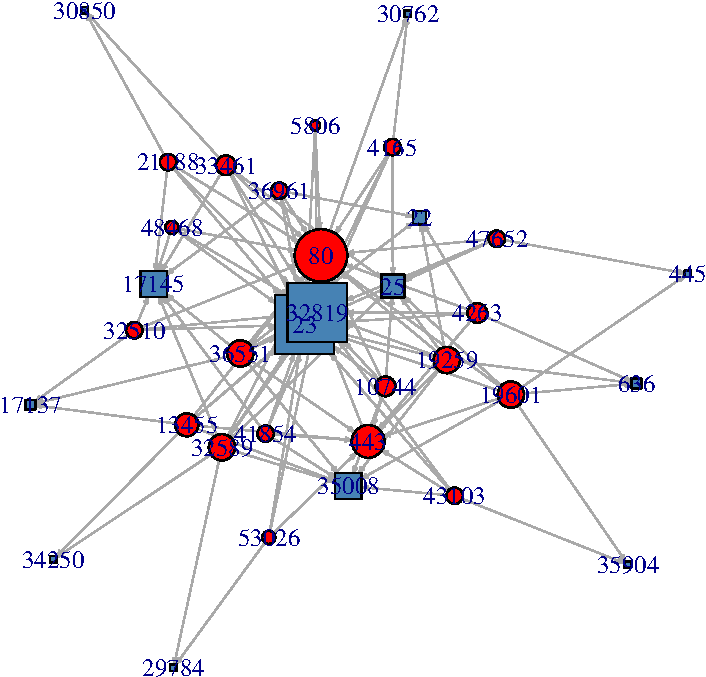
\includegraphics{thesis_files/figure-latex/unnamed-chunk-3-1.pdf}
\begin{Shaded}
\begin{Highlighting}[]
\KeywordTok{plot}\NormalTok{(ports_mean_matrix[!}\KeywordTok{is.na}\NormalTok{(ports_mean_matrix)], filled[!}\KeywordTok{is.na}\NormalTok{(ports_mean_matrix)],}
     \DataTypeTok{xlim =} \KeywordTok{c}\NormalTok{(}\DecValTok{0}\NormalTok{,}\DecValTok{5000}\NormalTok{), }\DataTypeTok{ylim =} \KeywordTok{c}\NormalTok{(}\DecValTok{0}\NormalTok{,}\DecValTok{5000}\NormalTok{))}
\end{Highlighting}
\end{Shaded}
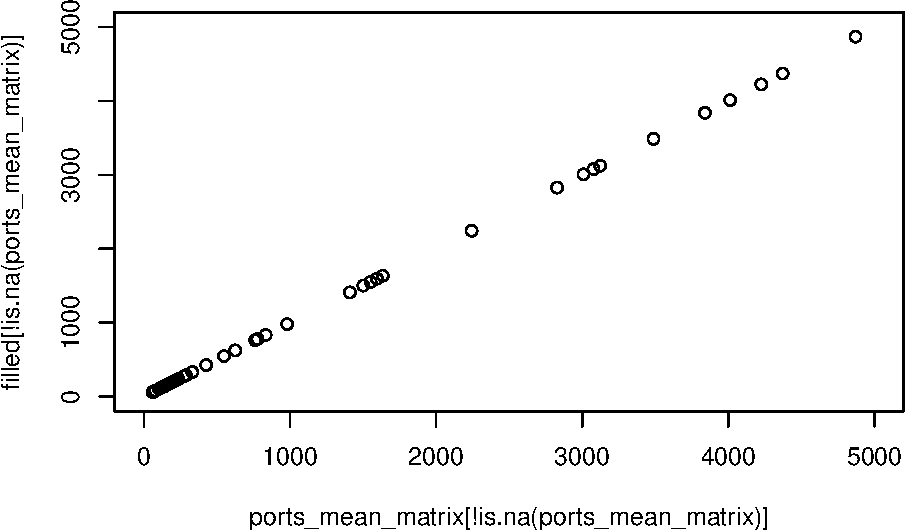
\includegraphics{thesis_files/figure-latex/unnamed-chunk-3-2.pdf}
\begin{Shaded}
\begin{Highlighting}[]
\NormalTok{####Eckhart Young Theorem Implementation, Best Rank k Approximation####}
\NormalTok{matrix_complete =}\StringTok{ }\NormalTok{function(}\DataTypeTok{S =} \DecValTok{1000}\NormalTok{, }\DataTypeTok{k =} \DecValTok{2}\NormalTok{, n_Sport, n_Dport, Y, M)\{}
  \NormalTok{S =}\StringTok{ }\DecValTok{1000}
  \NormalTok{k =}\StringTok{ }\DecValTok{2}
  \NormalTok{Y_imputed =}\StringTok{ }\NormalTok{Y}
  \CommentTok{#calculate overall mean}
  \NormalTok{n =}\StringTok{ }\DecValTok{0}
  \NormalTok{sum =}\StringTok{ }\DecValTok{0}
  \NormalTok{for (s in }\DecValTok{1}\NormalTok{:n_Sport)\{}
    \NormalTok{for (d in }\DecValTok{1}\NormalTok{:n_Dport)\{}
      \NormalTok{if (M[s,d] !=}\StringTok{ }\DecValTok{0}\NormalTok{)\{}
        \NormalTok{sum =}\StringTok{ }\NormalTok{sum +}\StringTok{ }\NormalTok{Y[s,d]}
        \NormalTok{n =}\StringTok{ }\NormalTok{n +}\StringTok{ }\NormalTok{M[s,d]}
      \NormalTok{\}}
    \NormalTok{\}}
  \NormalTok{\}}
  \NormalTok{overall_mean =}\StringTok{ }\NormalTok{sum/n}
  \CommentTok{#calculate row means and col means}
  \NormalTok{row_means =}\StringTok{ }\KeywordTok{rowMeans}\NormalTok{(Y, }\DataTypeTok{na.rm =} \OtherTok{TRUE}\NormalTok{)}
  \NormalTok{col_means =}\StringTok{ }\KeywordTok{colMeans}\NormalTok{(Y, }\DataTypeTok{na.rm =} \OtherTok{TRUE}\NormalTok{)}
  \CommentTok{#set NaN to 0 in means to fix anova fill in}
  \NormalTok{for (i in }\DecValTok{1}\NormalTok{:n_Sport)\{}
    \NormalTok{if (!}\KeywordTok{is.finite}\NormalTok{(row_means[i]))\{}
      \NormalTok{row_means[i] =}\StringTok{ }\DecValTok{0}
    \NormalTok{\}}
    \NormalTok{if (!}\KeywordTok{is.finite}\NormalTok{(col_means[i]))\{}
      \NormalTok{col_means[i] =}\StringTok{ }\DecValTok{0}
    \NormalTok{\}}
  \NormalTok{\}}
  \CommentTok{#Fill in missing values in Y_imputed with ANOVA}
  \NormalTok{for (s in }\DecValTok{1}\NormalTok{:n_Sport)\{}
    \NormalTok{for (d in }\DecValTok{1}\NormalTok{:n_Dport)\{}
      \NormalTok{if (M[s,d] ==}\StringTok{ }\DecValTok{0}\NormalTok{)\{}
        \NormalTok{Y_imputed[s,d] =}\StringTok{ }\NormalTok{row_means[s] +}\StringTok{ }\NormalTok{col_means[d] -}\StringTok{ }\NormalTok{overall_mean}
      \NormalTok{\}}
    \NormalTok{\}}
  \NormalTok{\}}
  \NormalTok{for (i in }\DecValTok{1}\NormalTok{:S)\{}
    \CommentTok{#extract SVD}
    \NormalTok{svd_Y =}\StringTok{ }\KeywordTok{svd}\NormalTok{(Y_imputed)}
    \NormalTok{D =}\StringTok{ }\KeywordTok{diag}\NormalTok{((svd_Y$d)[}\DecValTok{1}\NormalTok{:k])}
    \NormalTok{U =}\StringTok{ }\NormalTok{svd_Y$u}
    \NormalTok{V =}\StringTok{ }\NormalTok{svd_Y$v}
    \CommentTok{#EYM theorem}
    \NormalTok{EYM =}\StringTok{ }\NormalTok{U[,}\DecValTok{1}\NormalTok{:k] %*%}\StringTok{ }\NormalTok{D %*%}\StringTok{ }\KeywordTok{t}\NormalTok{(V[,}\DecValTok{1}\NormalTok{:k])}
    \CommentTok{#replace imputed values with new values, REPLACE ONLY MISSING OR REPLACE ALL? }
    \CommentTok{#Replacing only missing means we cant assess fitted error}
    \NormalTok{for (s in }\DecValTok{1}\NormalTok{:n_Sport)\{}
      \NormalTok{for (d in }\DecValTok{1}\NormalTok{:n_Dport)\{}
        \NormalTok{if (M[s,d] ==}\StringTok{ }\DecValTok{0}\NormalTok{)\{}
          \NormalTok{Y_imputed[s,d] =}\StringTok{ }\NormalTok{EYM[s,d]}
        \NormalTok{\}}
      \NormalTok{\}}
    \NormalTok{\}}
  \NormalTok{\}}
  \KeywordTok{return} \NormalTok{(Y_imputed)}
\NormalTok{\}}

\NormalTok{matrix_complete2 =}\StringTok{ }\NormalTok{function(Y, }\DataTypeTok{k =} \DecValTok{2}\NormalTok{, }\DataTypeTok{lambda =} \FloatTok{1.0}\NormalTok{)\{}
  \NormalTok{fit =}\StringTok{ }\KeywordTok{softImpute}\NormalTok{(Y, }\DataTypeTok{rank.max=}\NormalTok{k, }\DataTypeTok{lambda =} \NormalTok{lambda, }\DataTypeTok{trace=}\OtherTok{TRUE}\NormalTok{, }\DataTypeTok{type=}\StringTok{"als"}\NormalTok{)}
  \CommentTok{# fit$d}
  \NormalTok{filled =}\StringTok{ }\KeywordTok{complete}\NormalTok{(Y, fit)}
  \KeywordTok{return}\NormalTok{(filled)}
\NormalTok{\}}

\CommentTok{#ports_mean_matrix_imputed = matrix_complete(1000, 2, n_Sport, n_Dport, ports_mean_matrix, ports_freq_matrix)}

\CommentTok{#Relative distance using Frobenius Norm}
\NormalTok{relative_distance =}\StringTok{ }\NormalTok{function(Y, Y_imputed)\{}
  \KeywordTok{return} \NormalTok{(}\KeywordTok{frobenius.norm}\NormalTok{(Y -}\StringTok{ }\NormalTok{Y_imputed) /}\StringTok{ }\KeywordTok{frobenius.norm}\NormalTok{(Y))}
\NormalTok{\}}

\CommentTok{#Leave One Out Cross Validation}
\NormalTok{loocv =}\StringTok{ }\NormalTok{function (}\DataTypeTok{S =} \DecValTok{1000}\NormalTok{, }\DataTypeTok{k =} \DecValTok{2}\NormalTok{, }\DataTypeTok{nrows =} \NormalTok{n_Sport, }\DataTypeTok{ncols =} \NormalTok{n_Dport, Y, M)\{}
  \NormalTok{error =}\StringTok{ }\DecValTok{0}
  \NormalTok{rmse =}\StringTok{ }\DecValTok{0}
  \NormalTok{n =}\StringTok{ }\DecValTok{0}
  \NormalTok{for (s in }\DecValTok{1}\NormalTok{:nrows)\{}
    \NormalTok{for (d in }\DecValTok{1}\NormalTok{:ncols)\{}
      \NormalTok{if (M[s,d] !=}\StringTok{ }\DecValTok{0}\NormalTok{)\{}
        \NormalTok{n =}\StringTok{ }\NormalTok{n +}\StringTok{ }\DecValTok{1}
        \CommentTok{# M_imputed = M}
        \CommentTok{# M_imputed[s,d] = 0}
        \CommentTok{# Y_imputed = matrix_complete(S, k, nrows, ncols, Y, M_imputed)}
        \NormalTok{true_sd =}\StringTok{ }\NormalTok{Y[s,d]}
        \NormalTok{Y[s,d] <-}\StringTok{ }\OtherTok{NA}
        \NormalTok{Y_imputed =}\StringTok{ }\KeywordTok{matrix_complete2}\NormalTok{(Y, k, }\FloatTok{0.9}\NormalTok{)}
        \NormalTok{error =}\StringTok{ }\NormalTok{error +}\StringTok{ }\KeywordTok{abs}\NormalTok{((Y_imputed[s,d] -}\StringTok{ }\NormalTok{true_sd))}
        \NormalTok{rmse =}\StringTok{ }\NormalTok{rmse +}\StringTok{ }\NormalTok{(Y_imputed[s,d] -}\StringTok{ }\NormalTok{true_sd)^}\DecValTok{2}
        \NormalTok{Y[s,d] =}\StringTok{ }\NormalTok{true_sd}
      \NormalTok{\}}
    \NormalTok{\}}
  \NormalTok{\}}
  \NormalTok{rmse =}\StringTok{ }\KeywordTok{sqrt}\NormalTok{(rmse/n)}
  \KeywordTok{return} \NormalTok{(}\KeywordTok{list}\NormalTok{(}\DataTypeTok{Error =} \NormalTok{error, }\DataTypeTok{RMSE =} \NormalTok{rmse, }\DataTypeTok{Observations =} \NormalTok{n))}
\NormalTok{\}}

\CommentTok{# ranks = seq(1,10,1)}
\CommentTok{# #RMSEs = lapply(seq(1,10,1), function(k) loocv(250,k,n_Sport, n_Dport, ports_mean_matrix, ports_freq_matrix)$RMSE)}
\CommentTok{# RMSEs = c()}
\CommentTok{# for (k in ranks)\{}
\CommentTok{#   print (k)}
\CommentTok{#   cv = loocv(250,k,n_Sport, n_Dport, ports_mean_matrix, ports_freq_matrix)}
\CommentTok{#   RMSEs = c(RMSEs, cv$RMSE)}
\CommentTok{# \}}
\CommentTok{# plot(ranks, RMSEs)}
\CommentTok{# }
\CommentTok{# cv1 = loocv(250,1,n_Sport, n_Dport, ports_mean_matrix, ports_freq_matrix)}
\CommentTok{# cv2 = loocv(250,2,n_Sport, n_Dport, ports_mean_matrix, ports_freq_matrix)}
\CommentTok{# cv3 = loocv(250,3,n_Sport, n_Dport, ports_mean_matrix, ports_freq_matrix)}
\CommentTok{# cv5 = loocv(250,5,n_Sport, n_Dport, ports_mean_matrix, ports_freq_matrix)}
\end{Highlighting}
\end{Shaded}
\subsection{Results}\label{results}

While matrix completion via singular value decomposition presents valid
missing value imputations, and the algorithm converges relatively
quickly, the error generated from leave one out cross validation
reflects that the imputation performs rather poorly for low rank
solutions to the data. Moreover, the errors are minimized at a rank
approximation of 3, but even at this rank, the errors are relatively
high considering the data was first normal transformed.

This poor performance may largely be due to the fact the algorithm does
not account for the variability in the number of observed solutions for
each cell being imputed. Unlike the Netflix Competition, in which each
cell of the matrix being completed contained only a single user rating
of a movie, the matrix in this problem contains the average of a
variable number of observations in each cell.

\chapter{Tensor Completion}\label{tensor-completion}

\section{Motivation}\label{motivation-2}

This approach to the anomaly detection problem reduces the dataset to
the values of the four continuous features, SrcBytes, SrcPkts, DstBytes,
DstPkts, observed across different source port and destination port
combinations. The data can be represented as a 3-dimensional tensor
\(Y \in \mathbb{R_{m \times n \times 4}}\) where \(m\) represents the
number of source ports, \(n\) represents the number of destination
ports, and \(4\) accounts for the four continuous features in the
dataset. Each cell, \(y_{ijk}\), contains the mean of all the
observations observed for source port, \(i\), and destination port
\(j\). In the cases where the combination of \(i\) and \(j\) is not
observed in the dataset, \(y_{ijk}\) is missing.

The goal of this project is to devise an optimal strategy for imputing
the missing cells in \(Y\) to create the completed tensor
\(Y' \in \mathbb{R_{m \times n \times 4}}\). As new observations are
observed for combinations of ports \(i\) and \(j\), the \(y'_{ijk}\)
values can be interpreted as an approximation for the expected behavior
for that particular port combination. Observations with continuous
features that are a certain threshold away from \(y'_{ijk}\) may be
marked as anomalies and investigated further.

\section{Imputation Strategy}\label{imputation-strategy}

The imputation strategy focuses on finding a low rank approximation for
\(Y\) when decomposing the tensor.

\subsection{CP Decomposition}\label{cp-decomposition}

The CP decomposition expresses the tensor as:
\[Y = \sum_{r=1}^Ru_r \cdotp v_r \cdotp w_r\] where \(r\) represents the
rank approximation, \(\cdotp\) denotes the outer product of tensors, and
\(u \in \mathbb{R_{m \times r}}\), \(v \in \mathbb{R_{n \times r}}\),
and \(w \in \mathbb{R_{4 \times r}}\). Each individual cell is
expressed: \[y_{ijk} = \sum_{r=1}^Ru_{ri} \cdotp v_{ri} \cdotp w_{ri}\]
Applying this decomposition yields the objective
\[min_{Y'}\|Y-Y'\|, Y' = \sum_{r=1}^R\lambda_r(u_r \cdotp v_r \cdotp w_r)\],
where \(lambda_r\) is the regularization penalty.

\subsection{Variable Sample Sizes}\label{variable-sample-sizes}

A traditional approach to tensor completion involves using alternating
least squares regression to impute the missing values after populating
them with some initial values. The next section applies this approach to
a 2-dimensional \(m \times n\) tensor that represents a cross-section
slice of \(Y\) that only includes one of the four continuous features.
\emph{include als section here, related work:
\url{https://arxiv.org/abs/1410.2596} (hastie fast als), application
netflix challenge}

While this approach yields a completed tensor, it does not account for
the fact that the means in each cell are calculated from a variable
number of observations. Furthermore it is not necessarily true that
\(n_{ijk} = n_{i'j'k'}\) or \(\sigma^2_{ijk} = \sigma^2_{i'j'k'}\) for
\(i \neq i', j \neq j', k \neq k'\).

We propose the following model:
\[y_{ijk} \sim N(\mu_{ijk}, \frac{\sigma^2_{ijk}}{n_{ijk}})\] where
\(\mu_{ijk}\) is the sample mean, \(n_{ijk}\) is the sample size, and
\(\sigma^2_{ijk}\) is the sample variance of observations for source
port \(i\), destination port \(j\), and continuous feature \(k\).

Substituting these values into the Gaussian probability density function
yields the likelihood:
\[\frac{n_{ijk}}{\sigma^2_{ijk}}\sum(\bar y_{ijk} - \mu_{ijk})^2\]

Applying the CP/PARAFAC decomposition \(u_{ijk}\) is re-expressed:
\[u_{ijk} = \sum_{r=1}^Ra_{ir}b_{jr}c_{kr}\]

Vectorizing the inputs in the likelihood yields:
\[\sum_j\sum_k[\bar y_{ijk} - a_i^T(b_i \cdotp c_k)]\frac{n_{ijk}}{\sigma^2_{ijk}} (1)\]
where \(a_i \in \mathbb{R_{m \times r}}\),
\(b_j \in \mathbb{R_{n \times r}}\), and
\(c_k \in \mathbb{R_{4 \times r}}\). Summing across \(j\) and \(k\) in
this case solves for the \(ith\) row slice of the tensor. How to notate
vectorization of \(y\)?

Recall the Residual Sum of Squares (RSS) of the likelihood for an
Ordinary Least Squares (OLS) regression is expressed:
\[\sum_l(y_l-B^Tx_l)^2\]

Adding a weight, \(w_l\) to the summation yields a Weighted Least
Squares problem (WLS) \[\sum_l^nw_l(y_l-\beta^Tx_l)^2 (2)\] that is
analagous to the vectorized likelihood equation (1) with
\(w_l = \frac{n_{ijk}}{\sigma^2_{ijk}}\), \(\beta = a_i\),
\(x = (b_j \cdotp c_k)\).

With this formulation its now possible to solve for the optimal values
for each slice \(a_i\) of the tensor.

Recall that in a traditional vectorized OLS,
\(y = X\beta + \sigma\epsilon\), where
\(y \in \mathbb{R_{n \times 1}}\), \(X \in \mathbb{R_{n \times p}}\),
\(\beta \in \mathbb{R_{p \times 1}}\), and
\(\\sigma\epsilon \in \mathbb{R_{n \times 1}}\). Solving the maximum
likelihood estimator of \(\beta\), gives
\(\hat \beta = (X^TX)^{-1}X^Ty\).

Applying this formulation to the weighted least squares gives
\(y = X\beta + W^{-\frac{1}{2}}\epsilon\). Solving for the weighted
least squares estimator gives \(\hat \beta = (X^TWX)^{-1}X^TWy\).

Repeating this estimation technique across each slice of the tensor
\(a_i\), \(b_j\), \(c_k\) results in a completed model for \(y_{ijk}\).

\section{Motivation}\label{motivation-3}

The previous section's results reflected the need for an imputation
strategy that accounted for the variability in the number of
observations observed for each port combination when imputing that
particular combination's cell. The following section constructs a
statistical model that takes frequency of observations for each cell
into account and repeatedly samples from that statistical model to
complete the matrix.

\section{AMMI Model}\label{ammi-model}

Additive Main Effects and Multiplicative Interaction Models (AMMI
models) provide a defined statistical model for each cell in the ports
matrix. In particular, the model combines the additive effects of the
initial ANOVA imputation with the multiplicative effects yielded from
singular value decomposition described in the previous section. More
importantly, the model also includes a variance term for each cell that
takes into account the differing frequency of observations in each port
combination. Applying the same mathematical notation as the previous
section, the model is formally expressed:
\[y_{i,j} = u + a_i + b_j + \mathbf{u_i}D\mathbf{v_j^T} + \sigma_{i,j}\epsilon_{i,j}\]
where \(sigma_{i,j}\) is the variance for the \(ith\) row \(jth\) column
in the ports combination matrix, and \(\epsilon \sim N(0,1)\).

\section{Gibbs Sampling}\label{gibbs-sampling}

Following the application of the AMMI model, Gibbs Sampling is used to
repeatedly generate samples from the statistical model, yielding an
approximate value for each cell.

\chapter*{Conclusion}\label{conclusion}
\addcontentsline{toc}{chapter}{Conclusion}

If we don't want Conclusion to have a chapter number next to it, we can
add the \texttt{\{-\}} attribute.

\textbf{More info}

And here's some other random info: the first paragraph after a chapter
title or section head \emph{shouldn't be} indented, because indents are
to tell the reader that you're starting a new paragraph. Since that's
obvious after a chapter or section title, proper typesetting doesn't add
an indent there.

\backmatter

\chapter*{References}\label{references}
\addcontentsline{toc}{chapter}{References}

\markboth{References}{References}

\noindent

\setlength{\parindent}{-0.20in} \setlength{\leftskip}{0.20in}
\setlength{\parskip}{8pt}

\hypertarget{refs}{}
\hypertarget{ref-angel2000}{}
Angel, E. (2000). \emph{Interactive computer graphics : A top-down
approach with opengl}. Boston, MA: Addison Wesley Longman.

\hypertarget{ref-angel2001}{}
Angel, E. (2001a). \emph{Batch-file computer graphics : A bottom-up
approach with quicktime}. Boston, MA: Wesley Addison Longman.

\hypertarget{ref-angel2002a}{}
Angel, E. (2001b). \emph{Test second book by angel}. Boston, MA: Wesley
Addison Longman.


% Index?

\end{document}
